%%%%%%%%%%%%%%%%%%%%%%%%%%%%%%%%%%%%%%%%%%%%%%%%%%%%%%%%%%
% Ping GCM
%%%%%%%%%%%%%%%%%%%%%%%%%%%%%%%%%%%%%%%%%%%%%%%%%%%%%%%%%%
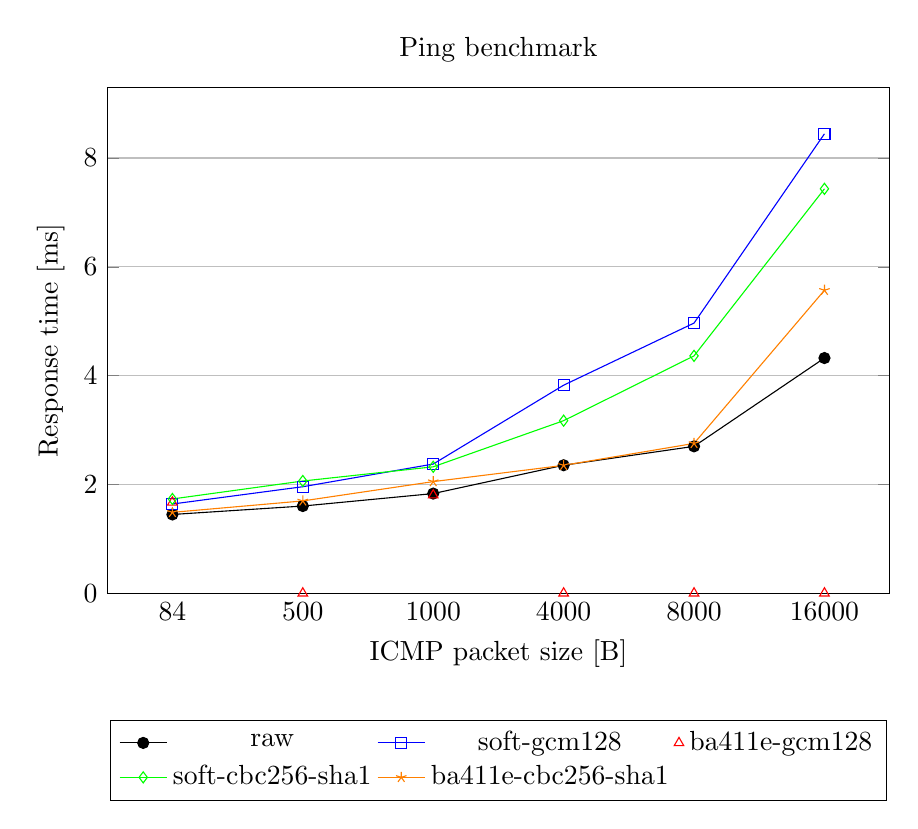
\begin{tikzpicture}
\begin{axis}[
        title = {Ping benchmark},
        width  = 0.95*\textwidth,
        height = 8cm,
        major x tick style = transparent,
        ymajorgrids = true,
        ylabel = {Response time [ms]},
        xlabel = {ICMP packet size [B]},
        ymin=0,
        xtick = data,
        symbolic x coords={84, 500, 1000, 4000, 8000, 16000},
        scaled ticks = false,%Disable the *10^4 exponent applied to all y axis markings.
        legend style={at={(0.5,-0.25)}, anchor=north,legend columns=3},
        % enlarge x limits=0.1,
    ]
% I would have prefered to have "\addplot[marks only]", but they overlap if they have the same x coordinate,
% not like bars that automatically shift.
\addplot[style={black, mark=*}]
    coordinates {
        (84,1.448)
        (500, 1.603)
        (1000,1.832)
        (4000, 2.353)
        (8000, 2.7)
        (16000, 4.323)
    };
    \label{raw}

\addplot[style={blue, mark=square}]
    coordinates {
        (84,1.640)
        (500, 1.958)
        (1000,2.375)
        (4000, 3.824)
        (8000, 4.966)
        (16000, 8.444)
    };
    \label{soft-gcm128}

\addplot[style={red, mark=triangle}, only marks]
    coordinates {
        (84,1.672)
        (500, 0)
        (1000,1.803)
        (4000, 0)
        (8000, 0)
        (16000, 0)
    };
    \label{ba411e-gcm128}

\addplot[style={green, mark=diamond}]
    coordinates {
        (84, 1.733)
        (500, 2.063)
        (1000, 2.324)
        (4000, 3.172)
        (8000, 4.363)
        (16000, 7.433)
    };
    \label{soft-cbc256-sha1}

\addplot[style={orange, mark=star}]
    coordinates {
        (84, 1.487)
        (500, 1.697)
        (1000, 2.052)
        (4000, 2.351)
        (8000, 2.754)
        (16000, 5.569)
    };
    \label{ba411e-cbc256-sha1}

\legend{raw, soft-gcm128, ba411e-gcm128, soft-cbc256-sha1, ba411e-cbc256-sha1}
\end{axis}
\end{tikzpicture}
% Here, I could show the gcm128, which show better performances with the BA411e, but I would be weird to compare it with aes256cbc.
% I need another graph with a CPu usage comparison to show that even if the perf are the same for soft/hard with aes256gcm, the hard loads less the CPU (I hope so, at least).